\begin{filecontents*}{em-test-refs.bib}
@book{griffiths2017,
  author    = {David J. Griffiths},
  title     = {Introduction to Electrodynamics},
  edition   = {4},
  publisher = {Cambridge University Press},
  year      = {2017}
}

@book{jackson1999,
  author    = {John David Jackson},
  title     = {Classical Electrodynamics},
  edition   = {3},
  publisher = {Wiley},
  year      = {1999}
}

@book{purcell2013,
  author    = {Edward M. Purcell and David J. Morin},
  title     = {Electricity and Magnetism},
  edition   = {3},
  publisher = {Cambridge University Press},
  year      = {2013}
}
\end{filecontents*}

\documentclass[11pt,a4paper]{article}

\usepackage[a4paper,margin=1in]{geometry}
\usepackage[T1]{fontenc}
\usepackage{lmodern}
\usepackage{microtype}

\usepackage{amsmath,amssymb,mathtools}
\usepackage{bm}
\usepackage{siunitx}
\usepackage{booktabs}
\usepackage{enumitem}
\usepackage{tikz}
\usetikzlibrary{arrows.meta,calc,decorations.pathmorphing,patterns}

\usepackage[
  backend=biber,
  style=ieee,
  sorting=none
]{biblatex}
\addbibresource{em-test-refs.bib}

\usepackage[colorlinks=true,linkcolor=blue,citecolor=magenta,urlcolor=teal]{hyperref}
\usepackage[nameinlink,noabbrev]{cleveref}

\setlength{\parskip}{0.5em}
\setlength{\parindent}{0pt}
\sisetup{per-mode=symbol}

\newcommand{\dd}{\mathop{}\!\mathrm{d}}
\newcommand{\ee}{\mathrm{e}}
\newcommand{\ii}{\mathrm{i}}
\newcommand{\vect}[1]{\bm{#1}}
\newcommand{\E}{\vect{E}}
\newcommand{\B}{\vect{B}}
\newcommand{\D}{\vect{D}}
\newcommand{\Hfield}{\vect{H}}
\newcommand{\J}{\vect{J}}
\newcommand{\A}{\vect{A}}
\newcommand{\grad}{\vect{\nabla}}
\newcommand{\curl}{\grad \times}
\newcommand{\divergence}{\grad \cdot}
\newcommand{\epszero}{\varepsilon_0}
\newcommand{\muzero}{\mu_0}

\title{Electromagnetism Test Document for VimTeX, SyncTeX, LSP, and Snippets}
\author{Generated Test File}
\date{\today}

\begin{document}
\maketitle

\begin{abstract}
This document is a deliberately equation-heavy electromagnetism sample for testing a LaTeX editing setup.
It includes cross-references, citations, displayed equations, aligned environments, a bibliography, TikZ figures, tables, labels, and enough page breaks to make forward and inverse SyncTeX testing meaningful.
Compile with \texttt{latexmk -pdf -synctex=1 em-test.tex}. 
For VimTeX, try \texttt{\textbackslash ll} to compile, \texttt{\textbackslash lv} to view, \texttt{\textbackslash le} for errors, and PDF-to-source inverse search in your viewer.
\end{abstract}

\tableofcontents
\newpage

\section{Electrostatics and Coulomb's Law}
\label{sec:electrostatics}

Electrostatics begins with the empirical observation that stationary charges exert forces on one another.
For point charges \(q_1\) and \(q_2\) separated by the vector \(\vect{r} = \vect{r}_1 - \vect{r}_2\), Coulomb's law is
\begin{equation}
  \vect{F}_{12}
  =
  \frac{1}{4\pi\epszero}
  \frac{q_1 q_2}{\lVert \vect{r} \rVert^2}
  \hat{\vect{r}} .
  \label{eq:coulomb-law}
\end{equation}
This is useful for force calculations, but field language is usually cleaner.
The electric field due to a point charge \(q\) at the origin is
\begin{equation}
  \E(\vect{r})
  =
  \frac{1}{4\pi\epszero}
  \frac{q}{r^2}\hat{\vect{r}} .
  \label{eq:point-charge-field}
\end{equation}
For a continuous charge distribution \(\rho(\vect{r}')\), the superposition principle gives
\begin{equation}
  \E(\vect{r})
  =
  \frac{1}{4\pi\epszero}
  \int_{\mathbb{R}^3}
  \rho(\vect{r}')
  \frac{\vect{r}-\vect{r}'}{\lVert \vect{r}-\vect{r}' \rVert^3}
  \dd^3 r' .
  \label{eq:field-integral}
\end{equation}

A useful test for editor navigation is to jump between \cref{eq:coulomb-law}, \cref{eq:point-charge-field}, and \cref{eq:field-integral}.
The conceptual move from forces to fields is emphasized in standard treatments such as \cite{griffiths2017,purcell2013}.

\subsection{Potential energy and electric potential}

Because the electrostatic field is conservative, it may be written as the negative gradient of a scalar potential:
\begin{equation}
  \E = -\grad V .
  \label{eq:electric-potential}
\end{equation}
The potential generated by a charge distribution is
\begin{equation}
  V(\vect{r})
  =
  \frac{1}{4\pi\epszero}
  \int
  \frac{\rho(\vect{r}')}{\lVert \vect{r}-\vect{r}' \rVert}
  \dd^3r' .
  \label{eq:potential-integral}
\end{equation}
This expression is often easier to evaluate than the vector integral in \cref{eq:field-integral}, after which the field can be recovered from \cref{eq:electric-potential}.

\begin{figure}[h]
\centering
\begin{tikzpicture}[scale=1.0]
  \draw[->] (-0.2,0) -- (5.2,0) node[right] {$x$};
  \draw[->] (0,-0.2) -- (0,3.2) node[above] {$y$};
  \filldraw[red] (1,1.5) circle (2.5pt) node[above left] {$q_1$};
  \filldraw[blue] (4,1.5) circle (2.5pt) node[above right] {$q_2$};
  \draw[thick,->] (1,1.5) -- (3.9,1.5) node[midway,above] {$\vect{r}_{12}$};
  \draw[dashed] (1,0) -- (1,1.5);
  \draw[dashed] (4,0) -- (4,1.5);
\end{tikzpicture}
\caption{Two point charges separated by a displacement vector. Use this figure to test SyncTeX jumps near captions, equations, and text.}
\label{fig:two-charges}
\end{figure}

See \cref{fig:two-charges} and test whether clicking near the caption in the PDF jumps to this source location.

\newpage

\section{Gauss's Law}
\label{sec:gauss}

Gauss's law is a compact expression of the relationship between electric flux and enclosed charge.
In integral form,
\begin{equation}
  \oint_{\partial \Omega} \E \cdot \dd \vect{a}
  =
  \frac{Q_{\mathrm{enc}}}{\epszero}.
  \label{eq:gauss-integral}
\end{equation}
Using the divergence theorem,
\begin{equation}
  \oint_{\partial \Omega} \E \cdot \dd \vect{a}
  =
  \int_{\Omega} \divergence \E \, \dd^3r,
\end{equation}
and since \(Q_{\mathrm{enc}} = \int_{\Omega}\rho \,\dd^3r\), one obtains the differential form
\begin{equation}
  \divergence \E = \frac{\rho}{\epszero}.
  \label{eq:gauss-differential}
\end{equation}

\subsection{Spherical symmetry}

For a point charge or uniformly charged sphere, symmetry forces the field to be radial:
\begin{equation}
  \E(\vect{r}) = E(r)\hat{\vect{r}}.
\end{equation}
A spherical Gaussian surface gives
\begin{align}
  \oint \E\cdot \dd\vect{a}
  &= E(r)4\pi r^2, \\
  E(r)4\pi r^2
  &= \frac{q}{\epszero}, \\
  E(r)
  &= \frac{1}{4\pi\epszero}\frac{q}{r^2}.
\end{align}
This recovers \cref{eq:point-charge-field}, but with far less calculation.

\subsection{Planar and cylindrical symmetry}

For an infinite charged sheet with surface charge density \(\sigma\), a pillbox Gaussian surface gives
\begin{equation}
  E = \frac{\sigma}{2\epszero}.
  \label{eq:sheet-field}
\end{equation}
For an infinite line charge with linear density \(\lambda\), a cylindrical Gaussian surface gives
\begin{equation}
  E(s) = \frac{\lambda}{2\pi\epszero s}.
  \label{eq:line-field}
\end{equation}
These examples are good places to test text-object motions, surrounding delimiters, and snippets for equations.

\begin{table}[h]
\centering
\caption{Common Gaussian surfaces and resulting electric fields.}
\label{tab:gaussian-fields}
\begin{tabular}{lll}
\toprule
Source & Gaussian surface & Field magnitude \\
\midrule
Point charge \(q\) & sphere & \(q/(4\pi\epszero r^2)\) \\
Infinite line \(\lambda\) & cylinder & \(\lambda/(2\pi\epszero s)\) \\
Infinite sheet \(\sigma\) & pillbox & \(\sigma/(2\epszero)\) \\
\bottomrule
\end{tabular}
\end{table}

\Cref{tab:gaussian-fields} is included to test table navigation, captions, and references.

\newpage

\section{Boundary Conditions and Conductors}
\label{sec:conductors}

In electrostatic equilibrium, the electric field inside a conductor is zero:
\begin{equation}
  \E_{\mathrm{inside}} = \vect{0}.
  \label{eq:conductor-inside}
\end{equation}
If this were not true, free charges would accelerate until they rearranged themselves to cancel the internal field.

The tangential component of the electrostatic field is continuous across a boundary:
\begin{equation}
  \hat{\vect{n}}\times(\E_2-\E_1)=\vect{0}.
  \label{eq:tangential-boundary}
\end{equation}
The normal component jumps by an amount determined by the surface charge density:
\begin{equation}
  \hat{\vect{n}}\cdot(\E_2-\E_1)
  =
  \frac{\sigma}{\epszero}.
  \label{eq:normal-boundary}
\end{equation}
Together, \cref{eq:tangential-boundary,eq:normal-boundary} are among the most useful local constraints in electrostatics.

\subsection{Capacitance}

For two conductors carrying charges \(+Q\) and \(-Q\), the capacitance is
\begin{equation}
  C = \frac{Q}{\Delta V}.
  \label{eq:capacitance-definition}
\end{equation}
For a parallel-plate capacitor with plate area \(A\) and separation \(d\), neglecting fringing fields,
\begin{equation}
  C = \frac{\epszero A}{d}.
  \label{eq:parallel-plate-capacitance}
\end{equation}
The stored electrostatic energy can be written as
\begin{equation}
  U = \frac{1}{2}CV^2
    = \frac{Q^2}{2C}
    = \frac{1}{2}Q V.
  \label{eq:capacitor-energy}
\end{equation}

\begin{figure}[h]
\centering
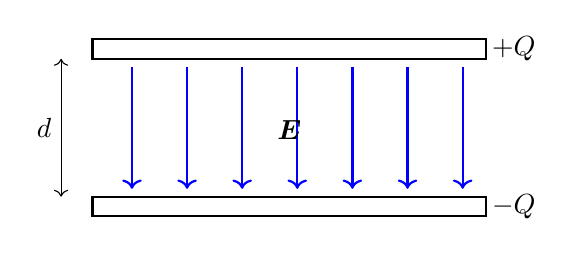
\begin{tikzpicture}[scale=1.0]
  \draw[thick] (0,0) rectangle (5,0.25);
  \draw[thick] (0,2) rectangle (5,2.25);
  \node at (5.35,0.125) {$-Q$};
  \node at (5.35,2.125) {$+Q$};
  \foreach \x in {0.5,1.2,1.9,2.6,3.3,4.0,4.7}
    \draw[->,blue,thick] (\x,1.9) -- (\x,0.35);
  \draw[<->] (-0.4,0.25) -- (-0.4,2) node[midway,left] {$d$};
  \node at (2.5,1.1) {$\E$};
\end{tikzpicture}
\caption{Idealized parallel-plate capacitor. The field is approximately uniform between the plates.}
\label{fig:parallel-plate}
\end{figure}

Try jumping from \cref{eq:parallel-plate-capacitance} to \cref{fig:parallel-plate} using your LSP or Telescope symbol tools.

\newpage

\section{Poisson and Laplace Equations}
\label{sec:poisson}

Combining \(\E = -\grad V\) with Gauss's law yields Poisson's equation:
\begin{equation}
  \nabla^2 V = -\frac{\rho}{\epszero}.
  \label{eq:poisson}
\end{equation}
In regions with no charge density, this reduces to Laplace's equation:
\begin{equation}
  \nabla^2 V = 0.
  \label{eq:laplace}
\end{equation}

\subsection{Uniqueness}

A central result is that solutions to Laplace's equation are unique once the boundary values are specified.
Suppose \(V_1\) and \(V_2\) both solve Laplace's equation in a region \(\Omega\) and agree on \(\partial\Omega\).
Define \(U = V_1 - V_2\). Then
\begin{equation}
  \nabla^2 U = 0,
  \qquad
  U|_{\partial\Omega}=0.
\end{equation}
Using Green's first identity,
\begin{equation}
  \int_{\Omega} \lVert \grad U\rVert^2 \dd^3 r
  =
  \oint_{\partial\Omega} U \grad U\cdot \dd\vect{a}
  -
  \int_{\Omega} U \nabla^2 U \dd^3 r
  =
  0.
\end{equation}
Therefore \(\grad U=\vect{0}\), and the boundary condition forces \(U=0\), so \(V_1=V_2\).

\subsection{Separation of variables}

In Cartesian coordinates,
\begin{equation}
  \nabla^2 V
  =
  \frac{\partial^2 V}{\partial x^2}
  +
  \frac{\partial^2 V}{\partial y^2}
  +
  \frac{\partial^2 V}{\partial z^2}.
\end{equation}
For a rectangular region, one may try
\begin{equation}
  V(x,y,z)=X(x)Y(y)Z(z),
\end{equation}
which turns the partial differential equation into ordinary differential equations.
This section is useful for testing snippets involving partial derivatives and aligned equations.

\begin{align}
  \frac{1}{X}\frac{\dd^2X}{\dd x^2}
  +
  \frac{1}{Y}\frac{\dd^2Y}{\dd y^2}
  +
  \frac{1}{Z}\frac{\dd^2Z}{\dd z^2}
  = 0.
  \label{eq:separation}
\end{align}

\newpage

\section{Magnetostatics}
\label{sec:magnetostatics}

Magnetostatics describes steady currents and time-independent magnetic fields.
The Lorentz force on a charge \(q\) moving with velocity \(\vect{v}\) is
\begin{equation}
  \vect{F}=q(\E+\vect{v}\times\B).
  \label{eq:lorentz-force}
\end{equation}
For a current distribution \(\J(\vect{r}')\), the Biot--Savart law gives
\begin{equation}
  \B(\vect{r})
  =
  \frac{\muzero}{4\pi}
  \int
  \J(\vect{r}')
  \times
  \frac{\vect{r}-\vect{r}'}
       {\lVert \vect{r}-\vect{r}'\rVert^3}
  \dd^3r'.
  \label{eq:biot-savart}
\end{equation}

\subsection{Ampere's law}

For steady currents, Ampere's law is
\begin{equation}
  \oint_{\partial S} \B\cdot \dd\vect{\ell}
  =
  \muzero I_{\mathrm{enc}}.
  \label{eq:ampere-integral}
\end{equation}
Using Stokes' theorem gives
\begin{equation}
  \curl \B = \muzero \J.
  \label{eq:ampere-differential}
\end{equation}
The magnetic field of a long straight wire follows immediately:
\begin{equation}
  B(s) = \frac{\muzero I}{2\pi s}.
  \label{eq:wire-field}
\end{equation}

\begin{figure}[h]
\centering
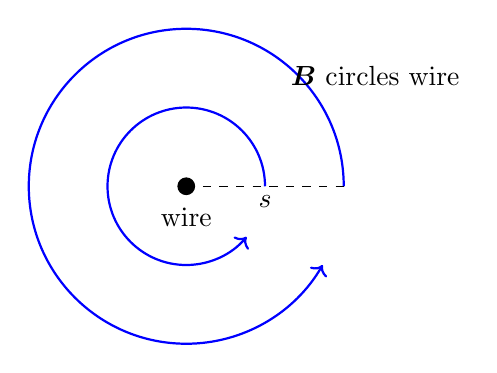
\begin{tikzpicture}[scale=1.0]
  \filldraw[black] (0,0) circle (3pt);
  \node[below] at (0,-0.15) {wire};
  \draw[blue,thick,->] (1,0) arc[start angle=0,end angle=320,radius=1];
  \draw[blue,thick,->] (2,0) arc[start angle=0,end angle=330,radius=2];
  \draw[dashed] (0,0) -- (2,0) node[midway,below] {$s$};
  \node at (2.4,1.4) {$\B$ circles wire};
\end{tikzpicture}
\caption{Magnetic field lines around a long straight current-carrying wire.}
\label{fig:wire-field}
\end{figure}

Magnetostatic calculations often mirror electrostatic ones, but with curls replacing divergences.
Compare \cref{eq:gauss-differential} with \cref{eq:ampere-differential}.

\newpage

\section{Vector Potential and Gauge Freedom}
\label{sec:vector-potential}

Because magnetic fields are solenoidal,
\begin{equation}
  \divergence \B = 0,
  \label{eq:no-monopoles}
\end{equation}
one may define a vector potential \(\A\) such that
\begin{equation}
  \B = \curl \A.
  \label{eq:vector-potential}
\end{equation}
The vector potential is not unique. If \(\chi\) is a scalar function, then
\begin{equation}
  \A' = \A + \grad \chi
\end{equation}
produces the same magnetic field because
\begin{equation}
  \curl \A'
  =
  \curl \A
  +
  \curl \grad \chi
  =
  \curl \A.
\end{equation}

\subsection{Coulomb gauge}

One common choice is the Coulomb gauge,
\begin{equation}
  \divergence \A = 0.
  \label{eq:coulomb-gauge}
\end{equation}
In magnetostatics, combining \cref{eq:ampere-differential,eq:vector-potential,eq:coulomb-gauge} yields
\begin{align}
  \curl(\curl\A)
  &=
  \grad(\divergence\A)-\nabla^2\A, \\
  -\nabla^2\A
  &=
  \muzero \J, \\
  \nabla^2\A
  &=
  -\muzero\J.
  \label{eq:vector-poisson}
\end{align}
This resembles Poisson's equation in \cref{eq:poisson}, but applies component-wise to the vector potential.

\subsection{Aharonov--Bohm intuition}

Even where \(\B = \vect{0}\), the vector potential may influence quantum phases.
This is one reason the vector potential is more than a mere computational convenience in quantum mechanics.
A classical electromagnetism course may introduce this only briefly, while more advanced treatments discuss it in detail \cite{jackson1999}.

\newpage

\section{Time-Dependent Fields and Maxwell's Correction}
\label{sec:time-dependent}

The magnetostatic form of Ampere's law is incomplete for time-dependent situations.
Taking the divergence of \(\curl\B=\muzero\J\) gives
\begin{equation}
  0 = \muzero \divergence \J,
\end{equation}
which would require charge conservation in the restricted form \(\divergence\J=0\).
But the continuity equation is
\begin{equation}
  \frac{\partial \rho}{\partial t} + \divergence\J = 0.
  \label{eq:continuity}
\end{equation}
Using Gauss's law,
\begin{equation}
  \rho = \epszero \divergence\E,
\end{equation}
the continuity equation becomes
\begin{equation}
  \divergence
  \left(
    \J + \epszero\frac{\partial\E}{\partial t}
  \right)
  =
  0.
\end{equation}
Maxwell's corrected Ampere law is therefore
\begin{equation}
  \curl \B
  =
  \muzero\J
  +
  \muzero\epszero
  \frac{\partial\E}{\partial t}.
  \label{eq:maxwell-ampere}
\end{equation}

\subsection{Faraday's law}

Faraday's law relates changing magnetic flux to induced electric fields:
\begin{equation}
  \oint_{\partial S}\E\cdot \dd\vect{\ell}
  =
  -
  \frac{\dd}{\dd t}
  \int_S \B\cdot\dd\vect{a}.
  \label{eq:faraday-integral}
\end{equation}
In differential form,
\begin{equation}
  \curl\E
  =
  -
  \frac{\partial\B}{\partial t}.
  \label{eq:faraday-differential}
\end{equation}
This is a good place to test diagnostics by intentionally deleting a brace, then using \texttt{\textbackslash le} to inspect errors.

\newpage

\section{Maxwell's Equations}
\label{sec:maxwell}

In vacuum with sources, Maxwell's equations are
\begin{align}
  \divergence \E
  &=
  \frac{\rho}{\epszero},
  \label{eq:maxwell-gauss-electric}
  \\
  \divergence \B
  &=
  0,
  \label{eq:maxwell-gauss-magnetic}
  \\
  \curl \E
  &=
  -
  \frac{\partial \B}{\partial t},
  \label{eq:maxwell-faraday}
  \\
  \curl \B
  &=
  \muzero\J
  +
  \muzero\epszero
  \frac{\partial\E}{\partial t}.
  \label{eq:maxwell-ampere-final}
\end{align}
Together these equations unify electrostatics, magnetostatics, induction, and electromagnetic waves.
The source-free case is obtained by setting \(\rho=0\) and \(\J=\vect{0}\).

\subsection{Constitutive relations}

In matter, it is often more useful to introduce \(\D\) and \(\Hfield\):
\begin{align}
  \D &= \epszero \E + \vect{P}, \\
  \Hfield &= \frac{1}{\muzero}\B - \vect{M}.
\end{align}
For simple linear media,
\begin{align}
  \D &= \varepsilon \E, \\
  \B &= \mu \Hfield.
\end{align}
Then the source equations become
\begin{align}
  \divergence \D &= \rho_{\mathrm{free}}, \\
  \curl \Hfield &= \J_{\mathrm{free}} + \frac{\partial \D}{\partial t}.
\end{align}

\begin{table}[h]
\centering
\caption{Differential Maxwell equations in vacuum.}
\label{tab:maxwell}
\begin{tabular}{ll}
\toprule
Equation & Meaning \\
\midrule
\(\divergence\E=\rho/\epszero\) & electric charge sources electric field \\
\(\divergence\B=0\) & no magnetic monopoles in classical EM \\
\(\curl\E=-\partial\B/\partial t\) & changing magnetic field induces electric circulation \\
\(\curl\B=\muzero\J+\muzero\epszero\partial\E/\partial t\) & current and displacement current source magnetic circulation \\
\bottomrule
\end{tabular}
\end{table}

Use \cref{tab:maxwell} to test citation, table, and reference completion.

\newpage

\section{Electromagnetic Waves}
\label{sec:waves}

In vacuum with no charges or currents, Maxwell's equations imply wave equations for both fields.
Taking the curl of Faraday's law gives
\begin{align}
  \curl(\curl\E)
  &=
  -
  \frac{\partial}{\partial t}
  (\curl\B), \\
  \grad(\divergence\E)-\nabla^2\E
  &=
  -
  \muzero\epszero
  \frac{\partial^2\E}{\partial t^2}.
\end{align}
Since \(\divergence\E=0\), this becomes
\begin{equation}
  \nabla^2\E
  -
  \muzero\epszero
  \frac{\partial^2\E}{\partial t^2}
  =
  0.
  \label{eq:e-wave}
\end{equation}
Similarly,
\begin{equation}
  \nabla^2\B
  -
  \muzero\epszero
  \frac{\partial^2\B}{\partial t^2}
  =
  0.
  \label{eq:b-wave}
\end{equation}
The wave speed is
\begin{equation}
  c = \frac{1}{\sqrt{\muzero\epszero}}.
  \label{eq:speed-of-light}
\end{equation}

\subsection{Plane waves}

A monochromatic plane wave propagating in the \(+\hat{\vect{z}}\) direction may be written
\begin{align}
  \E(z,t)
  &=
  E_0 \cos(kz-\omega t)\hat{\vect{x}},
  \\
  \B(z,t)
  &=
  \frac{E_0}{c}\cos(kz-\omega t)\hat{\vect{y}}.
\end{align}
The fields are transverse, mutually perpendicular, and related by
\begin{equation}
  \B = \frac{1}{c}\hat{\vect{k}}\times\E.
\end{equation}

\begin{figure}[h]
\centering
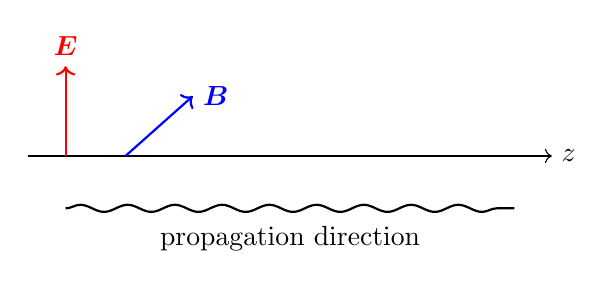
\begin{tikzpicture}[scale=0.95]
  \draw[->] (0,0) -- (7,0) node[right] {$z$};
  \draw[->,red,thick] (0.5,0) -- (0.5,1.2) node[above] {$\E$};
  \draw[->,blue,thick] (1.3,0) -- (2.2,0.8) node[right] {$\B$};
  \draw[decorate,decoration={snake,amplitude=0.45mm,segment length=6mm},thick]
    (0.5,-0.7) -- (6.5,-0.7);
  \node at (3.5,-1.1) {propagation direction};
\end{tikzpicture}
\caption{Schematic transverse electromagnetic plane wave.}
\label{fig:plane-wave}
\end{figure}

The derivation of \cref{eq:e-wave,eq:b-wave} is a useful stress test for equation alignment, references, and SyncTeX movement.

\newpage

\section{Energy, Momentum, and the Poynting Vector}
\label{sec:poynting}

The electromagnetic energy density in vacuum is
\begin{equation}
  u
  =
  \frac{1}{2}\epszero E^2
  +
  \frac{1}{2\muzero}B^2.
  \label{eq:energy-density}
\end{equation}
The Poynting vector is
\begin{equation}
  \vect{S}
  =
  \frac{1}{\muzero}
  \E\times\B.
  \label{eq:poynting-vector}
\end{equation}
It represents electromagnetic energy flux.

\subsection{Poynting theorem}

Starting from Maxwell's equations, one can derive
\begin{equation}
  \frac{\partial u}{\partial t}
  +
  \divergence\vect{S}
  =
  -
  \J\cdot\E.
  \label{eq:poynting-theorem}
\end{equation}
The term \(\J\cdot\E\) is the rate per unit volume at which fields do work on charges.
If \(\J=\vect{0}\), then electromagnetic energy is locally conserved:
\begin{equation}
  \frac{\partial u}{\partial t}
  +
  \divergence\vect{S}
  =
  0.
\end{equation}

\subsection{Radiation pressure}

Electromagnetic waves also carry momentum.
For a wave normally incident on a perfectly absorbing surface, the radiation pressure is
\begin{equation}
  p = \frac{\langle S\rangle}{c}.
\end{equation}
For a perfectly reflecting surface, the pressure doubles:
\begin{equation}
  p = \frac{2\langle S\rangle}{c}.
\end{equation}
This section is good for testing references to late-document equations such as \cref{eq:poynting-vector,eq:poynting-theorem}.

\newpage

\section{Potentials, Retardation, and a Final Checklist}
\label{sec:retarded}

For time-dependent fields, the scalar and vector potentials are often written
\begin{align}
  \E
  &=
  -\grad V
  -
  \frac{\partial\A}{\partial t},
  \label{eq:e-from-potentials}
  \\
  \B
  &=
  \curl\A.
  \label{eq:b-from-potentials}
\end{align}
In the Lorenz gauge,
\begin{equation}
  \divergence\A
  +
  \muzero\epszero
  \frac{\partial V}{\partial t}
  =
  0,
  \label{eq:lorenz-gauge}
\end{equation}
the potentials satisfy wave equations:
\begin{align}
  \nabla^2 V
  -
  \muzero\epszero
  \frac{\partial^2 V}{\partial t^2}
  &=
  -
  \frac{\rho}{\epszero},
  \\
  \nabla^2 \A
  -
  \muzero\epszero
  \frac{\partial^2 \A}{\partial t^2}
  &=
  -
  \muzero \J.
\end{align}
Their solutions are retarded potentials:
\begin{align}
  V(\vect{r},t)
  &=
  \frac{1}{4\pi\epszero}
  \int
  \frac{\rho(\vect{r}', t_r)}
       {\lVert \vect{r}-\vect{r}'\rVert}
  \dd^3r',
  \\
  \A(\vect{r},t)
  &=
  \frac{\muzero}{4\pi}
  \int
  \frac{\J(\vect{r}', t_r)}
       {\lVert \vect{r}-\vect{r}'\rVert}
  \dd^3r',
\end{align}
where
\begin{equation}
  t_r
  =
  t
  -
  \frac{\lVert \vect{r}-\vect{r}'\rVert}{c}.
  \label{eq:retarded-time}
\end{equation}

\subsection{Editing setup checklist}

Use this document to test the following workflow items:
\begin{enumerate}[label=\arabic*.]
  \item Compile continuously with \texttt{\textbackslash ll}.
  \item Open or forward-search the PDF with \texttt{\textbackslash lv}.
  \item Jump from PDF back to source using inverse SyncTeX.
  \item Inspect LaTeX errors with \texttt{\textbackslash le}.
  \item Open VimTeX information with \texttt{\textbackslash li} or \texttt{:VimtexInfo}.
  \item Search symbols such as \texttt{Maxwell} and \texttt{Poynting} with Telescope or LSP document symbols.
  \item Test snippets inside math zones, for example fractions, hats, bars, bras, kets, and display equations.
  \item Test citations such as \cite{griffiths2017}, \cite{purcell2013}, and \cite{jackson1999}.
\end{enumerate}

\subsection{Deliberate navigation targets}

Here are some source locations that should be easy to find from the PDF:
\begin{itemize}
  \item \Cref{eq:coulomb-law}: Coulomb's law.
  \item \Cref{eq:gauss-differential}: Gauss's law in differential form.
  \item \Cref{eq:biot-savart}: Biot--Savart law.
  \item \Cref{eq:maxwell-ampere-final}: Maxwell--Ampere law.
  \item \Cref{eq:e-wave}: electromagnetic wave equation.
  \item \Cref{eq:poynting-vector}: Poynting vector.
  \item \Cref{eq:retarded-time}: retarded time.
\end{itemize}

\printbibliography

\end{document}
